\documentclass{csbeamer}

\usepackage{dsfont}
\usepackage{amsmath}
\usepackage{amssymb}

% Add custom color definitions for MDPs
\definecolor{mdpmain}{HTML}{2E7D32}
\definecolor{mdpaccent}{HTML}{FF6B35}
\definecolor{mdplight}{HTML}{81C784}
\definecolor{mdpsecondary}{HTML}{1565C0}
\definecolor{mdpstate}{HTML}{4CAF50}
\definecolor{mdpaction}{HTML}{FF9800}
\definecolor{mdpreward}{HTML}{E91E63}
\definecolor{mdptransition}{HTML}{9C27B0}

\university{St. Francis Xavier University}
\department{Department of Computer Science}
\course{CSCI-531 - Reinforcement Learning}
\courseshort{CSCI-531 - RL}
\term{Fall 2025}
\author{Dr. Jean-Alexis Delamer}

\title{Markov Decision Processes}

\begin{document}

\frame{\titlepage}

% Section: From Bandits to Sequential Decisions
\section{Introduction}

\subsection{From Bandits to Sequential Decisions}

\begin{frame}
    \frametitle{Beyond Multi-Armed Bandits}

    \begin{block}<1->{Bandits vs. Real-World Decisions}
        \begin{itemize}
            \item<1-> \textcolor{mdpmain}{\textbf{Bandits}}: Each action is independent
            \item<2-> \textcolor{mdpaccent}{\textbf{Real World}}: Actions have lasting consequences
        \end{itemize}
    \end{block}

    \begin{block}<3->{Real-World Examples}
        \begin{itemize}
            \item<3-> \textbf{Robot Learning}: Each step affects balance for future steps
            \item<4-> \textbf{Drug Discovery}: Molecular modifications affect entire research trajectory
            \item<5-> \textbf{Language Model Training}: Each decision influences thousands of future steps
            \item<6-> \textbf{Algorithmic Trading}: Every trade changes portfolio state and risk
        \end{itemize}
    \end{block}

    \only<7->{
        \begin{center}
            \textcolor{mdpsecondary}{\textbf{These are sequential decision processes with ripple effects through time}}
        \end{center}
    }
\end{frame}

\begin{frame}
    \frametitle{The Challenge of Sequential Decisions}

    \begin{columns}
        \begin{column}{0.6\textwidth}
            \begin{block}<1->{Key Differences from Bandits}
                \begin{itemize}
                    \item<1-> \textcolor{mdpstate}{\textbf{State matters}}: Current situation affects future options
                    \item<2-> \textcolor{mdpaction}{\textbf{Actions have consequences}}: Choices change the world
                    \item<3-> \textcolor{mdpreward}{\textbf{Delayed rewards}}: Must trade off immediate vs future gains
                    \item<4-> \textcolor{mdptransition}{\textbf{Uncertainty}}: Outcomes are probabilistic
                \end{itemize}
            \end{block}
        \end{column}

        \begin{column}{0.4\textwidth}
            \begin{tikzpicture}[scale=1]
                % Robot navigation example
                \only<1->{
                    % Grid world
                    \draw[step=0.8cm,gray,very thin] (0,0) grid (2.4,2.4);

                    % Robot position
                    \draw[fill=mdpmain] (0.4,0.4) circle (0.2);
                    \node at (0.4,0.1) {\tiny Robot};

                    % Goal
                    \draw[fill=mdpreward] (2,2) circle (0.2);
                    \node at (2,1.7) {\tiny Goal};
                }

                \only<2->{
                    % Possible actions
                    \draw[->, thick, mdpaction] (0.4,0.6) -- (0.4,1.0);
                    \draw[->, thick, mdpaction] (0.6,0.4) -- (1.0,0.4);
                }

                \only<3->{
                    % Future consequences
                    \draw[dashed, mdpsecondary] (1.2,0.4) circle (0.15);
                    \draw[dashed, mdpsecondary] (0.4,1.2) circle (0.15);

                    \node at (1.5,-0.2) {\tiny Future states};
                }
            \end{tikzpicture}
        \end{column}
    \end{columns}

    \only<5->{
        \begin{center}
            \large{\textcolor{mdpmain}{\textbf{We need a mathematical framework for sequential decisions}}}
        \end{center}
    }
\end{frame}

% Section: MDP Definition
\section{Markov Decision Process Definition}

\subsection{Core Components}

\begin{frame}
    \frametitle{What is a Markov Decision Process?}

    \begin{block}<1->{MDP: Mathematical Framework}
        A Markov Decision Process models sequential decision-making under uncertainty
    \end{block}

    \begin{block}<2->{Key Properties}
        \begin{itemize}
            \item<2-> \textcolor{mdpmain}{\textbf{Sequential}}: Multiple decisions over time
            \item<3-> \textcolor{mdpaccent}{\textbf{Consequential}}: Each action affects future situations
            \item<4-> \textcolor{mdpsecondary}{\textbf{Uncertain}}: Outcomes are probabilistic
            \item<5-> \textcolor{mdpreward}{\textbf{Goal-oriented}}: Maximize long-term reward
        \end{itemize}
    \end{block}

    \only<6->{
        \begin{center}
            \textcolor{mdpmain}{\textbf{MDPs provide the foundation for virtually all modern RL algorithms}}
        \end{center}
    }
\end{frame}

\begin{frame}
    \frametitle{Formal MDP Definition}

    \begin{block}<1->{MDP Tuple $(S, A, T, R)$}
        \begin{itemize}
            \item<1-> $S$: Finite set of \textcolor{mdpstate}{\textbf{states}} (all possible situations)
            \item<2-> $A$: Finite set of \textcolor{mdpaction}{\textbf{actions}} (all choices available)
            \item<3-> $T: S \times A \times S \rightarrow [0,1]$: \textcolor{mdptransition}{\textbf{Transition function}} (world's physics)
            \item<4-> $R: S \times A \rightarrow \mathbb{R}$: \textcolor{mdpreward}{\textbf{Reward function}} (immediate feedback)
        \end{itemize}
    \end{block}

    \begin{center}
        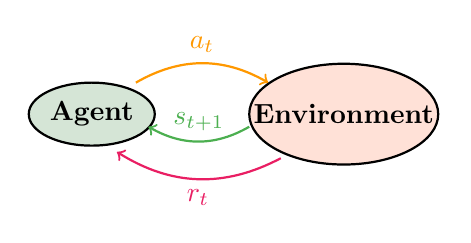
\begin{tikzpicture}[scale=0.8]
            \only<5->{
                % Agent-Environment interaction

                % Agent
                \draw[thick, fill=mdpmain!20] (0,1) ellipse (1 and 0.5);
                \node at (0,1) {\textbf{Agent}};

                % Environment
                \draw[thick, fill=mdpaccent!20] (4,1) ellipse (1.5 and 0.8);
                \node at (4,1) {\textbf{Environment}};

                % Action arrow
                \draw[->, thick, mdpaction] (0.7,1.5) to[bend left] node[above] {$a_t$} (2.8,1.5);

                % State and reward arrows
                \draw[->, thick, mdpstate] (2.5,0.8) to[bend left] node[above] {$s_{t+1}$} (0.9,0.8);
                \draw[->, thick, mdpreward] (3,0.3) to[bend left] node[below] {$r_t$} (0.4,0.4);
            }
        \end{tikzpicture}
    \end{center}
\end{frame}

\begin{frame}
    \frametitle{The Agent-Environment Interaction Loop}

    \begin{center}
        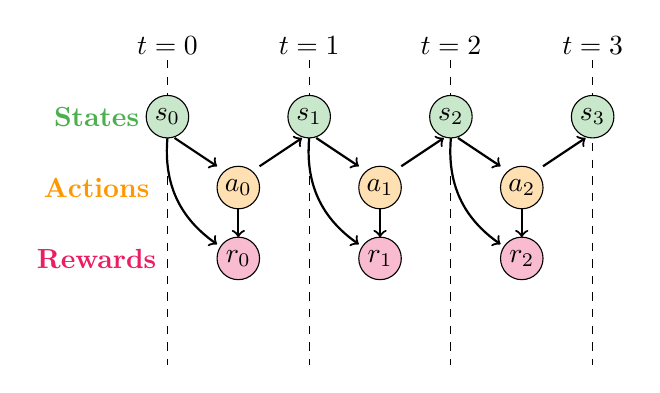
\begin{tikzpicture}[scale=0.9]
            % Timeline
            \foreach \t in {0,1,2,3} {
                \node at (2*\t,4) {$t=\t$};
                \draw[dashed] (2*\t,3.8) -- (2*\t,-0.5);
            }

            % States
            \foreach \t in {0,1,2,3} {
                \draw[fill=mdpstate!30] (2*\t,3) circle (0.3);
                \node at (2*\t,3) {$s_{\t}$};
            }

            % Actions
            \foreach \t in {0,1,2} {
                \draw[fill=mdpaction!30] (2*\t+1,2) circle (0.3);
                \node at (2*\t+1,2) {$a_{\t}$};
            }

            % Rewards
            \foreach \t in {0,1,2} {
                \draw[fill=mdpreward!30] (2*\t+1,1) circle (0.3);
                \node at (2*\t+1,1) {$r_{\t}$};
            }

            % Arrows
            \foreach \t in {0,1,2} {
                % State to action
                \draw[->, thick] (2*\t+0.1,2.7) -- (2*\t+0.7,2.3);
                % Action to next state
                \draw[->, thick] (2*\t+1.3,2.3) -- (2*\t+1.9,2.7);
                % Action to reward
                \draw[->, thick] (2*\t+1,1.7) -- (2*\t+1,1.3);
                % State to reward
                \draw[->, thick] (2*\t,2.7) to [bend right] (2*\t+0.7,1.2);
            }

            % Labels
            \node at (-1,3) {\textcolor{mdpstate}{\textbf{States}}};
            \node at (-1,2) {\textcolor{mdpaction}{\textbf{Actions}}};
            \node at (-1,1) {\textcolor{mdpreward}{\textbf{Rewards}}};
        \end{tikzpicture}
    \end{center}

    \begin{block}<2->{Trajectory Generation}
        This process generates a \textcolor{mdpmain}{\textbf{trajectory}} or \textbf{episode}:
        \begin{equation*}
            s_0, a_0, r_0, s_1, a_1, r_1, s_2, a_2, r_2, \ldots
        \end{equation*}
    \end{block}
\end{frame}

\subsection{Transition Function and Markov Property}

\begin{frame}
    \frametitle{Transition Function: The World's Physics}

    \begin{block}<1->{Probabilistic Transitions}
        After taking action $a_t$ in state $s_t$, next state $s_{t+1}$ is determined by:
        \begin{equation*}
            p(s'|s,a) = \text{Probability of moving to state } s' \text{ given state } s \text{ and action } a
        \end{equation*}
    \end{block}

    \begin{columns}
        \begin{column}{0.6\textwidth}
            \begin{block}<2->{Why Probabilistic?}
                \begin{itemize}
                    \item<2-> \textbf{Robot motors}: Have noise and uncertainty
                    \item<3-> \textbf{Market conditions}: Can change unexpectedly
                    \item<4-> \textbf{Experiments}: May have measurement errors
                    \item<5-> \textbf{Real world}: Is inherently stochastic
                \end{itemize}
            \end{block}
        \end{column}

        \begin{column}{0.4\textwidth}
            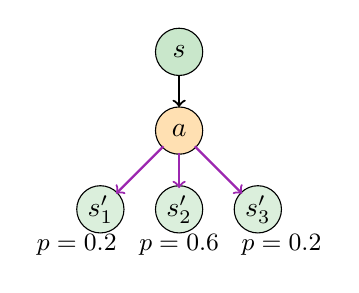
\begin{tikzpicture}
                \only<2->{
                    % Current state
                    \draw[fill=mdpstate!30] (1,2) circle (0.3);
                    \node at (1,2) {$s$};

                    % Action
                    \draw[fill=mdpaction!30] (1,1) circle (0.3);
                    \node at (1,1) {$a$};

                    % Possible next states
                    \draw[fill=mdpstate!20] (0,0) circle (0.3);
                    \node at (0,0) {$s_1'$};
                    \draw[fill=mdpstate!20] (1,0) circle (0.3);
                    \node at (1,0) {$s_2'$};
                    \draw[fill=mdpstate!20] (2,0) circle (0.3);
                    \node at (2,0) {$s_3'$};

                    % Transition probabilities
                    \draw[->, thick] (1,1.7) -- (1,1.3);
                    \draw[->, thick, mdptransition] (0.8,0.8) -- (0.2,0.2);
                    \draw[->, thick, mdptransition] (1,0.72) -- (1,0.27);
                    \draw[->, thick, mdptransition] (1.2,0.8) -- (1.8,0.2);

                    \node at (-0.3,-0.45) {\small $p=0.2$};
                    \node at (1,-0.45) {\small $p=0.6$};
                    \node at (2.3,-0.45) {\small $p=0.2$};
                }
            \end{tikzpicture}
        \end{column}
    \end{columns}

    \only<6->{
        \begin{center}
            Note: $\sum_{s' \in S} p(s'|s,a) = 1$ for all $s \in S, a \in A$
        \end{center}
    }
\end{frame}

\begin{frame}
    \frametitle{The Markov Property}

    \begin{block}<1->{Markov Property Definition}
        \textcolor{mdpmain}{\textbf{The future depends only on the present, not on the past}}

        Formally: All information needed to predict future states must be contained in the current state.
    \end{block}

    \begin{block}<2->{Mathematical Expression}
        \begin{equation*}
            P(S_{t+1} = s' | S_t = s_t, A_t = a_t, S_{t-1} = s_{t-1}, \ldots, S_0 = s_0) = P(S_{t+1} = s' | S_t = s_t, A_t = a_t)
        \end{equation*}
    \end{block}

    \begin{block}<3->{Examples}
        \begin{itemize}
            \item<3-> \textcolor{mdpmain}{\textbf{Markovian}}: Chess position (complete board state)
            \item<4-> \textcolor{mdpaccent}{\textbf{Non-Markovian}}: "Take the third turn" (depends on path history)
        \end{itemize}
    \end{block}
\end{frame}

\subsection{Reward Function}

\begin{frame}
    \frametitle{Reward Function: The Learning Signal}

    \begin{block}<1->{Reward Function Purpose}
        $r(s,a)$ provides immediate feedback that guides the agent toward its goal
    \end{block}

    \begin{block}<2->{Design Principles}
        \begin{itemize}
            \item<2-> Rewards communicate \textcolor{mdpmain}{\textbf{what}} to achieve, not \textbf{how}
            \item<3-> Given immediately after each action
            \item<4-> Should guide toward desired behavior
            \item<5-> \textcolor{mdpaccent}{\textbf{Warning}}: Poor design can lead to unintended behaviors!
        \end{itemize}
    \end{block}

    \begin{block}<6->{Common Examples}
        \begin{itemize}
            \item<6-> \textbf{Robot navigation}: $r = -1$ per step, $+100$ for goal
            \item<7-> \textbf{Game playing}: $r = +1$ win, $-1$ loss, $0$ otherwise
        \end{itemize}
    \end{block}
\end{frame}

% Section: Cumulative Rewards and Returns
\section{Returns and Value Functions}

\subsection{Cumulative Rewards}

\begin{frame}
    \frametitle{From Immediate to Cumulative Rewards}

    \begin{block}<1->{The Challenge}
        \begin{itemize}
            \item<1-> Actions have lasting consequences
            \item<2-> We care about \textcolor{mdpmain}{\textbf{total}} reward over time, not just immediate
            \item<3-> Future outcomes are uncertain due to stochastic transitions
        \end{itemize}
    \end{block}

    \begin{center}
        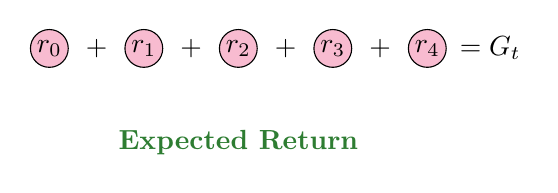
\begin{tikzpicture}[scale=0.8]
            \only<4->{
                % Reward sequence
                \foreach \t in {0,1,2,3,4} {
                    \draw[fill=mdpreward!30] (\t*1.5,1) circle (0.3);
                    \node at (\t*1.5,1) {$r_{\t}$};
                }

                % Plus signs
                \foreach \t in {0,1,2,3} {
                    \node at (\t*1.5+0.75,1) {$+$};
                }

                % Equals
                \node at (7,1) {$= G_t$};

                \node at (3,-0.5) {\textcolor{mdpmain}{\textbf{Expected Return}}};
            }
        \end{tikzpicture}
    \end{center}

    \begin{block}<5->{Return Definition}
        The \textcolor{mdpmain}{\textbf{return}} $G_t$ is the cumulative reward from time $t$:
        \begin{equation*}
            G_t = r_t + r_{t+1} + r_{t+2} + \cdots + r_T
        \end{equation*}
    \end{block}
\end{frame}

\begin{frame}
    \frametitle{The Problem with Infinite Horizons}

    \begin{block}<1->{What if $T = \infty$?}
        \begin{itemize}
            \item<2-> Sum might blow up to infinity
            \item<3-> Cannot compare different strategies
            \item<4-> Need a solution for continuing tasks
        \end{itemize}
    \end{block}

    \begin{block}<5->{Solution: Discounted Return}
        Introduce \textcolor{mdpmain}{\textbf{discount factor}} $\gamma \in [0,1]$:
        \begin{equation*}
            G_t = r_t + \gamma r_{t+1} + \gamma^2 r_{t+2} + \cdots = \sum_{k=0}^{\infty} \gamma^k r_{t+k}
        \end{equation*}
    \end{block}
\end{frame}

\begin{frame}
    \frametitle{The Problem with Infinite Horizons}

    \begin{block}<1->{Discounted Return}
        Introduce \textcolor{mdpmain}{\textbf{discount factor}} $\gamma \in [0,1]$:
        \begin{equation*}
            G_t = r_t + \gamma r_{t+1} + \gamma^2 r_{t+2} + \cdots = \sum_{k=0}^{\infty} \gamma^k r_{t+k}
        \end{equation*}
    \end{block}

    \begin{block}<2->{Discount Factor Interpretation}
        \begin{itemize}
            \item<3-> $\gamma = 0$: Only immediate rewards matter (completely myopic)
            \item<4-> $\gamma = 1$: All future rewards equally important (completely farsighted)
            \item<5-> $\gamma = 0.9$: Future rewards matter, but less than immediate ones
        \end{itemize}
    \end{block}
\end{frame}

\begin{frame}
    \frametitle{Discount Factor Example}

    \begin{columns}
        \begin{column}{0.6\textwidth}
            \textbf{Scenario}: Receive reward of 10 at each time step

            \textbf{With $\gamma = 0.5$}:
            \begin{align*}
                G_0 &= 10 + 0.5 \times 10 + 0.5^2 \times 10 + \cdots \\
                &= 10 + 5 + 2.5 + 1.25 + \cdots \\
                &= \frac{10}{1-0.5} = 20
            \end{align*}

            \textbf{With $\gamma = 0.9$}:
            \begin{align*}
                G_0 &= 10 + 9 + 8.1 + 7.29 + \cdots \\
                &= \frac{10}{1-0.9} = 100
            \end{align*}
        \end{column}

        \begin{column}{0.4\textwidth}
            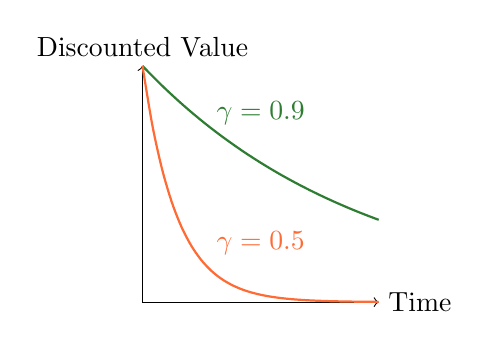
\begin{tikzpicture}[scale=0.3]
                % Discount visualization
                \draw[->] (0,0) -- (10,0) node[right] {Time};
                \draw[->] (0,0) -- (0,10) node[above] {Discounted Value};

                % γ = 0.9 curve
                \draw[thick, mdpmain] plot [smooth, domain=0:10] (\x, {0.9^\x*10)});
                \node at (5,8) {\textcolor{mdpmain}{$\gamma = 0.9$}};

                % γ = 0.5 curve
                \draw[thick, mdpaccent] plot [smooth, domain=0:10] (\x, {0.5^\x*10)});
                \node at (5,2.5) {\textcolor{mdpaccent}{$\gamma = 0.5$}};
            \end{tikzpicture}
        \end{column}
    \end{columns}

    \only<2->{
        \begin{center}
            \textcolor{mdpsecondary}{\textbf{Higher $\gamma$ values future rewards more}}
        \end{center}
    }
\end{frame}

\subsection{Policies and Value Functions}

\begin{frame}
    \frametitle{Policies: Decision-Making Strategies}

    \begin{block}<1->{Policy Definition}
        A \textcolor{mdpmain}{\textbf{policy}} $\pi$ is a mapping from states to action probabilities:
        \begin{equation*}
            \pi(a|s) = \text{Probability of selecting action } a \text{ in state } s
        \end{equation*}
    \end{block}

    \begin{columns}
        \begin{column}{0.6\textwidth}
            \begin{block}<2->{Types of Policies}
                \begin{itemize}
                    \item<2-> \textcolor{mdpmain}{\textbf{Deterministic}}: $\pi(a|s) \in \{0,1\}$
                        \begin{itemize}
                            \item Always same action in same state
                        \end{itemize}
                    \item<3-> \textcolor{mdpaccent}{\textbf{Stochastic}}: $\pi(a|s) \in (0,1)$
                        \begin{itemize}
                            \item Probabilistic action selection
                        \end{itemize}
                \end{itemize}
            \end{block}
        \end{column}

        \begin{column}{0.4\textwidth}
            \begin{tikzpicture}[scale=1]
                \only<2->{
                    % Grid world example
                    \draw[step=0.8cm,gray,very thin] (0,0) grid (2.4,1.6);

                    % States
                    \foreach \x in {0,1,2} {
                        \foreach \y in {0,1} {
                            \draw[fill=mdpstate!20] (0.4+\x*0.8,0.4+\y*0.8) circle (0.15);
                        }
                    }

                    % Policy arrows (deterministic)
                    \only<2>{
                        \draw[->, thick, mdpmain] (0.4,0.4) -- (0.4,0.7);
                        \draw[->, thick, mdpmain] (1.2,0.4) -- (1.5,0.4);
                        \draw[->, thick, mdpmain] (2.0,0.4) -- (2.0,0.7);
                        \draw[->, thick, mdpmain] (0.4,1.2) -- (0.7,1.2);
                        \draw[->, thick, mdpmain] (1.2,1.2) -- (1.5,1.2);
                    }

                    % Policy arrows (stochastic)
                    \only<3>{
                        \draw[->, mdpaccent, thick] (0.4,0.4) -- (0.4,0.7);
                        \draw[->, mdpaccent, thick] (0.4,0.4) -- (0.7,0.4);
                        \node at (0.1,0.6) {\tiny 0.7};
                        \node at (0.6,0.1) {\tiny 0.3};
                    }
                }
            \end{tikzpicture}
        \end{column}
    \end{columns}

    \only<4->{
        \begin{center}
            \textcolor{mdpsecondary}{\textbf{A policy completely specifies the agent's behavior}}
        \end{center}
    }
\end{frame}

\begin{frame}
    \frametitle{Value Functions: Evaluating Policies}

    \begin{block}<1->{State Value Function}
        The \textcolor{mdpmain}{\textbf{value}} of state $s$ under policy $\pi$:
        \begin{equation*}
            v_\pi(s) = \mathbb{E}_\pi[G_t | S_t = s] = \mathbb{E}_\pi\left[\sum_{k=0}^{\infty} \gamma^k r_{t+k} \bigg| S_t = s\right]
        \end{equation*}

        \textit{"Expected return when starting in state $s$ and following policy $\pi$"}
    \end{block}

    \begin{block}<2->{Action-Value Function (Q-Function)}
        The \textcolor{mdpaccent}{\textbf{value}} of taking action $a$ in state $s$ under policy $\pi$:
        \begin{equation*}
            q_\pi(s,a) = \mathbb{E}_\pi[G_t | S_t = s, A_t = a] = \mathbb{E}_\pi\left[\sum_{k=0}^{\infty} \gamma^k r_{t+k} \bigg| S_t = s, A_t = a\right]
        \end{equation*}

        \textit{"Expected return when taking action $a$ in state $s$, then following policy $\pi$"}
    \end{block}

\end{frame}

\begin{frame}
    \frametitle{Value Functions: Evaluating Policies}

    \begin{block}{State Value Function}
        \begin{equation*}
            v_\pi(s) = \mathbb{E}_\pi[G_t | S_t = s] = \mathbb{E}_\pi\left[\sum_{k=0}^{\infty} \gamma^k r_{t+k} \bigg| S_t = s\right]
        \end{equation*}

    \end{block}

    \begin{block}{Action-Value Function (Q-Function)}
        \begin{equation*}
            q_\pi(s,a) = \mathbb{E}_\pi[G_t | S_t = s, A_t = a] = \mathbb{E}_\pi\left[\sum_{k=0}^{\infty} \gamma^k r_{t+k} \bigg| S_t = s, A_t = a\right]
        \end{equation*}
    \end{block}

    \only<2->{
        \begin{center}
            \textcolor{mdpsecondary}{\textbf{Relationship}}: $v_\pi(s) = \sum_a \pi(a|s) q_\pi(s,a)$
        \end{center}
    }
\end{frame}

\begin{frame}
    \frametitle{Bellman Equation: The Key Recursive Relationship}

    \begin{block}<1->{Bellman Equation Derivation}
        \begin{align*}
            v_\pi(s) &= \mathbb{E}_\pi[G_t | S_t = s] \\
            \onslide<2->{&= \mathbb{E}_\pi[r_t + \gamma G_{t+1} | S_t = s] \\}
            \onslide<3->{&= \sum_a \pi(a|s) \sum_{s'} p(s'|s,a) [r(s,a) + \gamma \mathbb{E}_\pi[G_{t+1} | S_{t+1} = s']] \\}
            \onslide<4->{&= \sum_a \pi(a|s) \sum_{s'} p(s'|s,a) [r(s,a) + \gamma v_\pi(s')]}
        \end{align*}
    \end{block}
\end{frame}

\begin{frame}
    \frametitle{Bellman Equation: The Key Recursive Relationship}

    \begin{block}{Bellman Equation Derivation}
        \begin{align*}
            v_\pi(s) = \sum_a \pi(a|s) \sum_{s'} p(s'|s,a) [r(s,a) + \gamma v_\pi(s')]
        \end{align*}
    \end{block}

    \begin{block}<2->{Interpretation}
        \begin{itemize}
            \item<2-> \textcolor{mdpreward}{\textbf{Immediate reward}}: $r(s,a)$
            \item<3-> \textcolor{mdpmain}{\textbf{Future value}}: $\gamma v_\pi(s')$ (discounted)
            \item<4-> \textcolor{mdptransition}{\textbf{Weighted by probabilities}}: Policy and transitions
        \end{itemize}
    \end{block}
\end{frame}

% Section: Optimal Policies and Value Functions
\section{Optimal Policies and Value Functions}

\subsection{Finding the Best Policy}

\begin{frame}
    \frametitle{Optimal Policies and Value Functions}

    \begin{block}<1->{Policy Comparison}
        Policy $\pi$ is \textcolor{mdpmain}{\textbf{better than}} policy $\pi'$ if:
        \begin{equation*}
            v_\pi(s) \geq v_{\pi'}(s) \text{ for all states } s \in S
        \end{equation*}
    \end{block}

    \begin{block}<2->{Fundamental Theorem}
        \textcolor{mdpmain}{\textbf{There always exists at least one optimal policy}} that is better than or equal to all other policies.
    \end{block}
\end{frame}

\begin{frame}
    \frametitle{Optimal Policies and Value Functions}

    \begin{block}{Optimal Value Functions}
        \textbf{Optimal state value function}:
        \begin{equation*}
            v^*(s) = \max_\pi v_\pi(s) \text{ for all } s \in S
        \end{equation*}

        \textbf{Optimal action-value function}:
        \begin{equation*}
            q^*(s,a) = \max_\pi q_\pi(s,a) \text{ for all } s \in S, a \in A
        \end{equation*}
    \end{block}
\end{frame}

\begin{frame}
    \frametitle{Bellman Optimality Equations}

    \begin{block}<1->{Bellman Optimality Equation for $v^*$}
        \begin{align*}
            v^*(s) &= \max_a q^*(s,a) \\
            &= \max_a \mathbb{E}[r_{t+1} + \gamma v^*(S_{t+1}) | S_t = s, A_t = a] \\
            &= \max_a \sum_{s'} p(s'|s,a)[r(s,a) + \gamma v^*(s')]
        \end{align*}
    \end{block}

    \begin{block}<2->{Key Insight}
        Instead of averaging over policy probabilities, we take the \textcolor{mdpmain}{\textbf{maximum}} over all possible actions.
    \end{block}
\end{frame}

\begin{frame}
    \frametitle{Bellman Optimality Equations}

    \begin{block}<1->{Bellman Optimality Equation for $v^*$}
        \begin{align*}
            v^*(s) &= \max_a q^*(s,a) \\
            &= \max_a \sum_{s'} p(s'|s,a)[r(s,a) + \gamma v^*(s')]
        \end{align*}
    \end{block}

    \begin{block}<2->{Finding the Optimal Policy}
        Once we have $v^*$, the optimal policy is:
        \begin{equation*}
            \pi^*(s) = \arg\max_a \sum_{s'} p(s'|s,a)[r(s,a) + \gamma v^*(s')]
        \end{equation*}

        \textit{Choose the action that achieves the maximum in the Bellman optimality equation}
    \end{block}
\end{frame}

\begin{frame}
    \frametitle{MDP Solution Methods}

    \begin{block}<1->{Dynamic Programming Methods}
        When we know the MDP model $(S, A, T, R)$:
        \begin{itemize}
            \item<1-> \textcolor{mdpmain}{\textbf{Policy Iteration}}: Alternate between policy evaluation and improvement
            \item<2-> \textcolor{mdpaccent}{\textbf{Value Iteration}}: Iteratively update value function using Bellman optimality equation
            \item<3-> \textcolor{mdpsecondary}{\textbf{Guaranteed convergence}} to optimal policy
        \end{itemize}
    \end{block}

    \begin{block}<4->{When Model is Unknown}
        Real-world applications often don't know transition probabilities:
        \begin{itemize}
            \item<4-> \textcolor{mdpmain}{\textbf{Model-free RL}}: Learn from experience without knowing $T$ or $R$
            \item<5-> \textcolor{mdpaccent}{\textbf{Temporal Difference Learning}}: Update estimates using observed transitions
            \item<6-> \textcolor{mdpsecondary}{\textbf{Q-Learning, SARSA}}: Popular algorithms for this setting
        \end{itemize}
    \end{block}
\end{frame}

% Section: MDP Applications
\section{MDP Applications}

\subsection{Real-World Applications}

\begin{frame}
    \frametitle{MDP Applications in Modern AI}

    \begin{block}<1->{Computational Biology \& Drug Discovery}
        \begin{itemize}
            \item<1-> \textcolor{mdpstate}{\textbf{State}}: Molecular configuration, binding sites, chemical properties
            \item<2-> \textcolor{mdpaction}{\textbf{Actions}}: Add/remove functional groups, modify structure
            \item<3-> \textcolor{mdpreward}{\textbf{Reward}}: Binding affinity, toxicity, synthesis complexity
            \item<4-> \textcolor{mdpaccent}{\textbf{Challenge}}: Massive state spaces, sparse rewards
        \end{itemize}
    \end{block}

    \begin{block}<5->{Advanced Robotics}
        \begin{itemize}
            \item<5-> \textcolor{mdpstate}{\textbf{State}}: Joint positions, velocities, environment perception
            \item<6-> \textcolor{mdpaction}{\textbf{Actions}}: Motor commands, grasp planning, trajectory selection
            \item<7-> \textcolor{mdpreward}{\textbf{Reward}}: Task completion, energy efficiency, safety
            \item<8-> \textcolor{mdpaccent}{\textbf{Challenge}}: Continuous spaces, real-time constraints
        \end{itemize}
    \end{block}
\end{frame}

\begin{frame}
    \frametitle{Advanced MDP Applications}

    \begin{block}<1->{Large Language Model Training}
        \begin{itemize}
            \item<1-> \textcolor{mdpstate}{\textbf{State}}: Model parameters, training data batch, loss landscape
            \item<2-> \textcolor{mdpaction}{\textbf{Actions}}: Learning rate adjustments, architecture modifications
            \item<3-> \textcolor{mdpreward}{\textbf{Reward}}: Validation performance, computational efficiency
            \item<4-> \textcolor{mdpaccent}{\textbf{Challenge}}: Non-stationary environments, delayed feedback
        \end{itemize}
    \end{block}

    \begin{block}<5->{Research Strategy Optimization}
        \begin{itemize}
            \item<5-> \textcolor{mdpstate}{\textbf{State}}: Current knowledge, available resources, progress
            \item<6-> \textcolor{mdpaction}{\textbf{Actions}}: Experiment design, resource allocation, collaborations
            \item<7-> \textcolor{mdpreward}{\textbf{Reward}}: Scientific impact, knowledge gain, progress metrics
            \item<8-> \textcolor{mdpaccent}{\textbf{Challenge}}: Extremely long horizons, uncertain outcomes
        \end{itemize}
    \end{block}
\end{frame}

\subsection{MDP Formulation Skills}

\begin{frame}
    \frametitle{Key Skills: MDP Formulation}

    \begin{block}<1->{Problem Formulation Process}
        \begin{enumerate}
            \item<1-> \textcolor{mdpstate}{\textbf{Define State Space}}: What information is crucial for decisions?
            \item<2-> \textcolor{mdpaction}{\textbf{Action Space}}: What decisions can you make? Discrete vs continuous?
            \item<3-> \textcolor{mdptransition}{\textbf{Transition Dynamics}}: How do actions change states? What's uncertain?
            \item<4-> \textcolor{mdpreward}{\textbf{Reward Design}}: How do you quantify progress toward goals?
            \item<5-> \textcolor{mdpaccent}{\textbf{Scalability}}: What makes this computationally challenging?
        \end{enumerate}
    \end{block}

    \begin{block}<6->{Critical Questions}
        \begin{itemize}
            \item<6-> Does your state representation satisfy the Markov property?
            \item<7-> Does your reward function capture what you actually want?
            \item<8-> Where might the MDP framework break down?
        \end{itemize}
    \end{block}
\end{frame}

% Section: Research Frontiers
\section{Looking Forward}

\subsection{MDP Challenges and Extensions}

\begin{frame}
    \frametitle{Current Research Challenges}

    \begin{block}<1->{Computational Challenges}
        \begin{itemize}
            \item<1-> \textcolor{mdpaccent}{\textbf{Curse of Dimensionality}}: State spaces grow exponentially
            \item<2-> \textcolor{mdpmain}{\textbf{Continuous Spaces}}: Real problems rarely have discrete states/actions
            \item<3-> \textcolor{mdpsecondary}{\textbf{Partial Observability}}: Perfect state information often unrealistic
        \end{itemize}
    \end{block}

    \begin{block}<4->{Research Frontiers}
        \begin{itemize}
            \item<4-> \textcolor{mdpmain}{\textbf{Transfer Learning}}: How do solutions generalize across problems?
            \item<5-> \textcolor{mdpaccent}{\textbf{Multi-Agent MDPs}}: What happens when multiple agents interact?
            \item<6-> \textcolor{mdpsecondary}{\textbf{Inverse RL}}: Can we infer reward functions from behavior?
            \item<7-> \textcolor{mdpreward}{\textbf{Safe RL}}: How to ensure safety during learning?
        \end{itemize}
    \end{block}
\end{frame}

\begin{frame}
    \frametitle{Summary}

    \begin{block}{What We've Learned}
        \begin{itemize}
            \item \textcolor{mdpmain}{\textbf{MDP Framework}}: States, actions, transitions, rewards
            \item \textcolor{mdpaccent}{\textbf{Sequential Decision Making}}: Actions have lasting consequences
            \item \textcolor{mdpsecondary}{\textbf{Value Functions}}: Evaluate policies and states
            \item \textcolor{mdpreward}{\textbf{Optimal Solutions}}: Bellman equations and dynamic programming
        \end{itemize}
    \end{block}

    \begin{block}{Next Steps}
        \begin{itemize}
            \item Dynamic Programming algorithms (Policy/Value Iteration)
            \item Model-free reinforcement learning
            \item Temporal difference learning
            \item Deep reinforcement learning
        \end{itemize}
    \end{block}

    \begin{center}
        \large{\textcolor{mdpmain}{\textbf{From bandits to MDPs: The foundation is complete!}}}
    \end{center}
\end{frame}

\end{document}
